\chapter{Collaborative Tasks}
\label{chapter:colab-tasks}

% Descrição geral deste capítulo das collaborative tasks





\section{Hand Guiding}

\par So far, it has been explained how to obtain a compensated \ac{ft} measurement in order to obtain \acf{hgft}, which is caused by the user. This value is used to move the robot in the direction that it is applied. For this to happen, this values felt on the \ac{ft} reference frame need to be converted to a velocity vector, referenced on the base frame of the robot. 



\subsection{\ac{hgft} to \ac{eef} Velocity}
\label{ssec:ft_to_eef}

\par \ac{hgft} should only converted in robot motion when it reaches a certain threshold, otherwise, it should be zero. It should also exist a way to define the ration of conversion between \ac{ft} and velocity To achieve this behavior, the \ac{hgft} is controlled according to \autoref{eq:f_thresh} and \autoref{eq:t_thresh}.

\begin{multicols}{2}
    \begin{equation}
        \mathbf{f_i} =
        \begin{cases}
          \frac{f_i - f_{th}}{f_{div}} & f_i > f_{th}\\
          \frac{f_i + f_{th}}{f_{div}} & f_i < f_{th}\\
          0 & \text{otherwise}
        \end{cases}
        \label{eq:f_thresh}
    \end{equation}\break
    \begin{equation}
        \mathbf{t_i} =
        \begin{cases}
          \frac{t_i - t_{th}}{t_{div}} & t_i > t_{th}\\
          \frac{t_i + t_{th}}{t_{div}} & t_i < t_{th}\\
          0 & \text{otherwise}
        \end{cases}
        \label{eq:t_thresh} 
    \end{equation}
\end{multicols}

\noindent Where $\mathbf{f_i}$ and $\mathbf{t_i}$ are \ac{ft} components, $\mathbf{t_{th}}$ and $\mathbf{f_{th}}$ are \ac{ft} threshold parameters, and $\mathbf{t_{div}}$ and $\mathbf{f_{div}}$ are ratio constants that define the conversion between \ac{ft} and velocity.

\subsubsection{Force to Linear Velocity}

\par It is done by creating a pose with the force measurement as the position component, and transforming this pose with the rotation matrix of the \ac{ft} sensor frame. The resulting pose position can be directly used as global velocity. \autoref{eq:force_to_linear_vel} is used to calculate the linear velocity from the \ac{hg} force.

\begin{equation}
    \vec{\mathbf{V_{lin}}} = R^b_e \cdot R^e_s \cdot P_{force}
    \label{eq:force_to_linear_vel}
\end{equation}

\noindent Where $\mathbf{R^b_e}$ is the rotation matrix of the \ac{eef} frame in relation to the robot base frame, $\mathbf{R^e_s}$ is a constant rotation matrix of the sensor frame in relation to the \ac{eef} frame, and $P_{force}$ is a point with the force measurements as its coordinates. $\vec{\mathbf{V_{lin}}}$ is obtained as a cartesian points which can directly be used as a linear velocity vector in the robot base frame.

\subsubsection{Torque to Angular Velocity}

\par It is done by creating a pose with the torque measurement as the orientation component, transforming this orientation with the rotation matrix of the \ac{ft} sensor frame, and with this orientation, rotate the inverse rotation of the \ac{ft} sensor frame. \autoref{eq:force_to_linear_vel} is used to calculate the angular velocity from the \ac{hg} torque.

\begin{equation}
    \vec{\mathbf{V_{ang}}} = (R^b_e \cdot R^e_s \cdot R_{torque}) \cdot (R^b_e \cdot R^e_s)^{-1}
    \label{eq:torque_to_angular_vel}
\end{equation}

\noindent Where $\mathbf{R^b_e}$ is the rotation matrix of the \ac{eef} frame in relation to the robot base frame, $\mathbf{R^e_s}$ is a constant rotation matrix of the sensor frame in relation to the \ac{eef} frame, and $R_{torque}$ is a rotation with the torque measurements as its elements. $\vec{\mathbf{V_{ang}}}$ is obtained as a cartesian rotation which can directly be used as angular velocity in the robot base frame.



\subsection{\ac{eef} Velocity to Joint Speed}
\label{ssec:eef_to_js}

\par With the previous equations, the \ac{eef} velocity in cartesian space is obtained from the \ac{hgft} on the \ac{ft} sensor. As said before, in this work, the \ac{ur10e} will be controlled in joint space with joint speed commands. To obtain joint speeds from an \ac{eef} velocity, the Jacobian inversion method will be used.

\subsubsection{Jacobian Inversion Method}

\par The Jacobian matrix is used in robotics to provide a relation between joint speeds and \ac{eef} velocities in a robotic manipulator. This relation is given by \autoref{eq:jacobian}.

\begin{equation}
    \dot{\mathbf{X}} = J(q)\dot{q}
    \label{eq:jacobian}
\end{equation}

\noindent Where $\dot{\mathbf{q}}$ is the robot joint velocities, $\mathbf{q}$ is the robot joint positions, $\mathbf{J}$ is the Jacobian matrix, which is a function of the current robot joint positions. $\dot{\mathbf{X}}$ represents the \ac{eef} velocity and is obtained in the form of a 1 column matrix with 6 elements. The first part represents linear velocity, and the second represent angular velocity. The Jacobian matrix is obtained through forward kinematics equations applied on a given joint state. In this work, the Jacobian matrix is obtained with the MoveIt motion planning framework, using the \ac{ur10e} robot description. 

\par In order to obtain joint speeds from the \ac{eef} velocities, the Jacobian matrix is inverted and \autoref{eq:inv_jacobian} is used.

\begin{equation}
    \dot{\mathbf{q}} = J(q)^{-1} \dot{X}
    \label{eq:inv_jacobian}
\end{equation}

\noindent Since the \ac{ur10e} has 6 joints, its Jacobian matrix is a square matrix, and it is possible to directly invert it and use it according to the previous equation to convert \ac{eef} velocities into joint speeds.



\subsection{\ac{hg} Architecture}

\par Having the joint speeds calculated, they are sent back to the ROS driver by publishing them into the appropriate topic, at 500Hz. The \ac{ros} architecture for this task is demonstrated in \autoref{fig:ros_hg_arch}.

\begin{figure}[h]
    \centering
    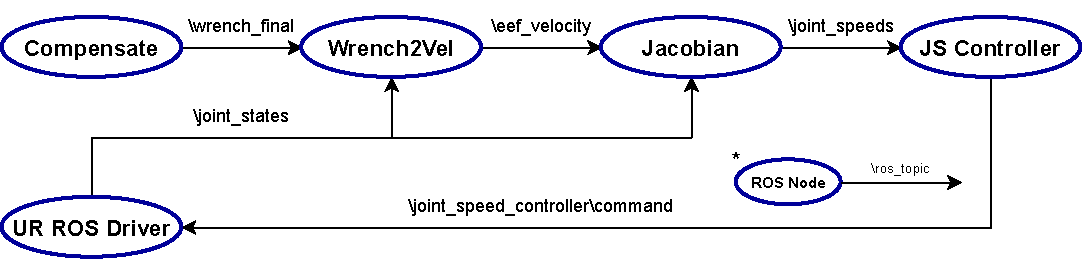
\includegraphics[width=\linewidth]{figs/chp5/ros_hg_arch.pdf}
    \caption{\ac{ros} architecture of the \ac{hg} task}
    \label{fig:ros_hg_arch}
\end{figure}

\par The Wrench2Vel \ac{ros} node implements the algorithms explained in \autoref{ssec:ft_to_eef} and the Jacobian node implements the Jacobian inversion method described in \autoref{ssec:eef_to_js}. The \ac{js} Controller node subscribes to the joint speeds calculated with the Jacobian matrix and publishes them in the appropriate topic made available by the \ac{ur} \ac{ros} driver. This node also implements a filter to smooth the robot acceleration when rapidly changing velocity, and a \ac{ros} service that allows its control with play, pause and stop functions.





\section{Object Transfer}

\par The object transfer collaborative task is an example of a user customizable skill. It is very similar to the general pick and place task with the only difference being that the final destination is not a place position, but rather a deliver position where the robot will wait for user input to release the object. This task has various states, and each state has input parameters and a certain behavior. \autoref{fig:object_transfer} shows the arrangement of the states and their parameters.

\begin{figure}[h]
    \centering
    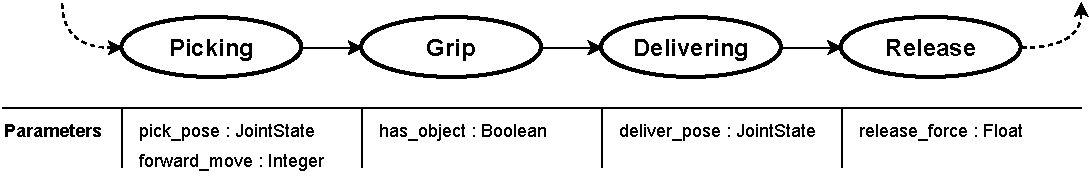
\includegraphics[width=\linewidth]{figs/chp5/pick_and_deliver.pdf}
    \caption{State architecture of the object transfer task}
    \label{fig:object_transfer}
\end{figure}

\par The task starts by moving the robot to a picking position, defined in the \textit{pick\_pose}. Since this position is a predefined joint state, the trajectory can planned with the MoveIt framework and the motion of the robot is controlled though its positional controller. This position is preferably a few centimeters distant from the object, so the next step is to move the robot forward according to the \textit{forward\_move} parameter.
\par The robot should reach the next state with its gripper fingers aligned with the object, therefore, the next step is to close the gripper. The \textit{has\_ojbect} flag is a control parameter used to only proceed in the flow of the task if the gripper has gripped anything. This happens if the flag is set to true, otherwise, the task continues ignoring if the gripper has gripped any object.
\par The Delivering state moves the robot to another predefined position. When it reaches that position, it automatically skips to the Release state, where it stops and the system continuously evaluates the \ac{ft} measured. If the \textit{release\_force} parameter is configured, the robot will release the object when a force with magnitude equal to \textit{release\_force} is applied. If this parameter is not set, which is the default behavior, the robot will release the object when its weight has been supported by the user, which programmatically means that the robot will release the object when the \ac{ft} measured in the Z-Axis of the world frame is higher than zero. 

% ADD: Capacidades deste tipo de task, descrição geral





\section{Object Manipulation}

\par The object manipulation task has the goal of allowing the user to give the robot an object and be able to \ac{hg} it with precision, while the robot holds the object. \autoref{fig:object_manipulation} shows the composition of this task states.

\begin{figure}[h]
    \centering
    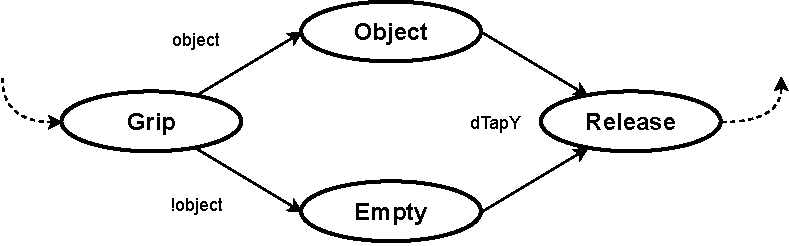
\includegraphics[width=0.7\linewidth]{figs/chp5/object_manipulation.pdf}
    \caption{State architecture of the object manipulation task}
    \label{fig:object_manipulation}
\end{figure}

\par The Grip state has been seen previously, but this time, instead of configuring a parameter to evaluate if the gripper has anything attached, this condition will be used as a way to determine the next state. It the gripper has no object, it will skip to the Empty state which has no internal behavior other that to wait for user input. This input has the form of a double tap on the \ac{eef}, in the Y-Axis direction. Further details on this communication interface with the system will be given in \autoref{ssec:double_tap}.
\par If the gripper has an object, the system will skip to the Object state where the attached Payload will be measured and injected in the theoretical \ac{ft} model. This state starts by turning of the velocity controller and moving the robot upwards. This motion serves as a signal to the user to not touch the \ac{eef} for a while. Then, the system obtains a \ac{ft} measure and from it, it calculates the object weight and \ac{cog}. With this parameters, it updates the theoretical \ac{ft} model through its \textbackslash\textit{payload\_update} \ac{ros} service. Once the theoretical \ac{ft} model gives confirmation, the velocity controller is turned back on, and with the updated values of payload, the user can accurately \ac{hg} the system knowing that it will compensate the object weight. When the user is done with this task, he executes the same double tap as explained before and the robot skips to the Release state.
\par Finally, in the Release state, the velocity controller is turned off, the robot releases the object, the theoretical \ac{ft} model is configured with just the gripper tool payload, the \ac{ft} sensor is tared, and just before leaving this state, the the velocity controller is resumed.

% Capacidades deste tipo de task, necessidade de andar sempre a ligar desligar o controlador de velocidade, cuz pesos e merdas






\section{Collision Free Execution of an Industrial Task}

\par This system allows for seamless integration of any industrial task given it provides a certain control interface. This control interface requires the existence of play, pause and stop services that will be called depending of user interaction. The structure of the states of this task can be seen in \autoref{fig:industrial_task}.

\begin{figure}[h]
    \centering
    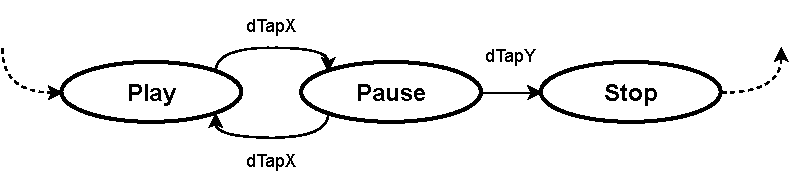
\includegraphics[width=0.7\linewidth]{figs/chp5/industrial_task.pdf}
    \caption{State architecture of the industrial task}
    \label{fig:industrial_task}
\end{figure}

\par In this Dissertation, the industrial task implemented is a looped transition between two positions with dynamic collision avoidance. Programmatically, when this state is activated, the behavior described in \autoref{chapter:obstacle} is reproduced in a loop by activating the \ac{apf} Controller node. The trajectory defined in the Planner node will start being executed and any obstacles detected by the Obstacles node will be avoided. While the task is executing, the user can pause it by approaching the \ac{eef}, which will start to slow down, and make a double tap on its X-Axis.





\section{Collaborative State Machine}

\par The tasks explained before are all arranged in a global state machine that treats each task as a submachine. The initial state is the Hand Guiding task which allows free manipulation of the robot. To execute a task, a double tap in a specific direction must be executed on the robot \ac{eef}. The behavior flow of the global state machine is described in \autoref{fig:ros_smach}.

\begin{figure}[h]
    \centering
    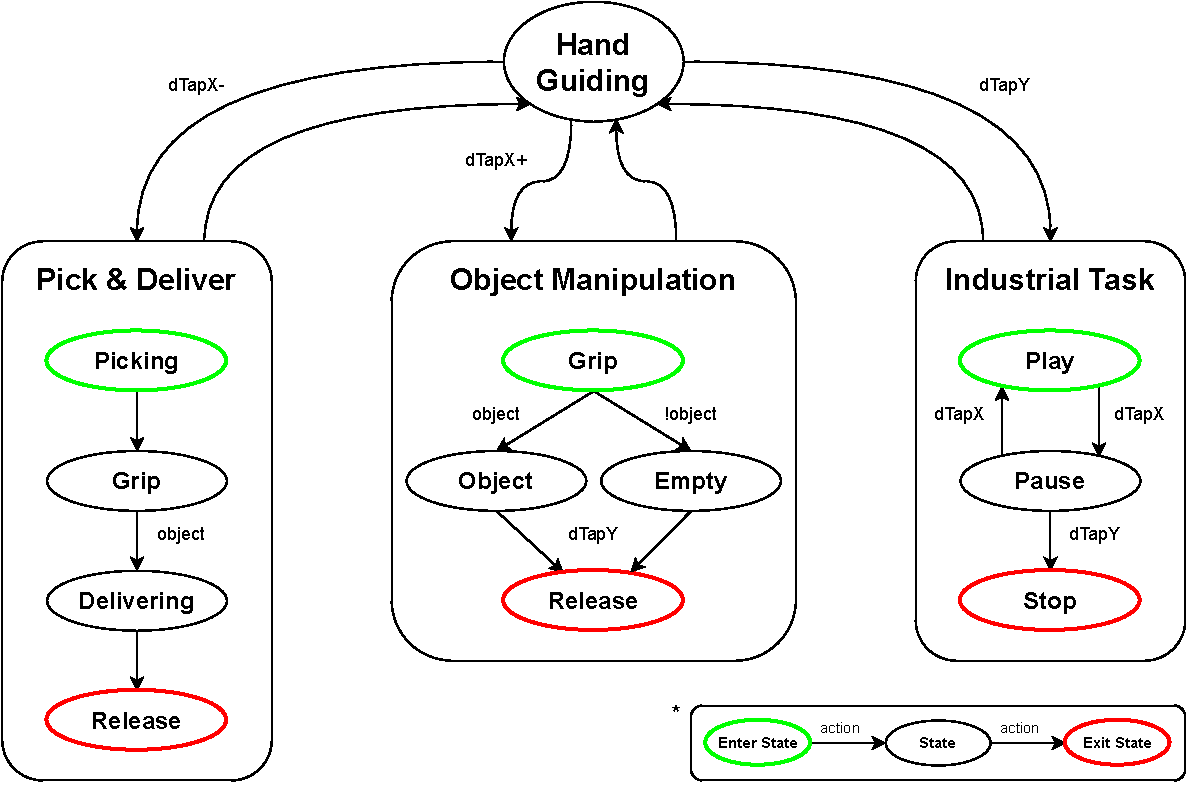
\includegraphics[width=0.8\linewidth]{figs/chp5/ros_ur10e_smach.pdf}
    \caption{Collaborative state machine}
    \label{fig:ros_smach}
\end{figure}

\par The integration of this tasks with each other is seamless. They all start from the \ac{hg} state and also return to it when finished. On of the main advantages of an arrangement such as this, is that in the execution of the different tasks the robot can be controlled by multiple entities. For instance, the Object Transfer task uses the MoveIt positional controller, the Object Manipulation uses the Wrench2Vel \ac{ros} node, and the Industrial Task uses the PF2Vel \ac{ros} node. The existence of a structure such as this state machine, allows for a cohesive and seamless change of control entities, without the user ever noticing their existence.

\begin{figure}[h]
    \centering
    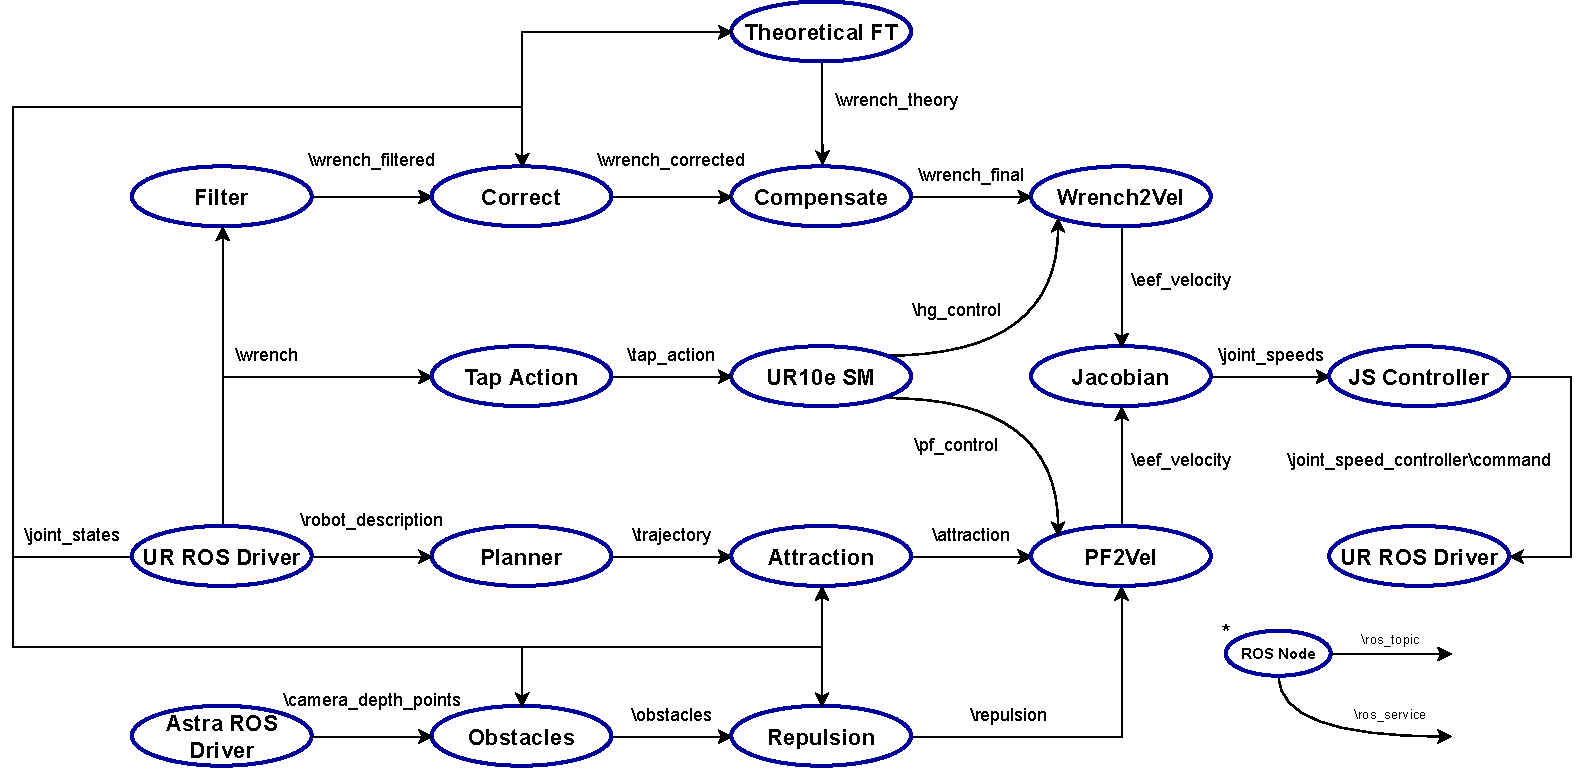
\includegraphics[width=\linewidth]{figs/chp5/ros_cobot_arch.pdf}
    \caption{Complete \ac{ros} architecture of the system}
    \label{fig:ros_cobot_arch}
\end{figure}

\par A complete view of the \ac{ros} architecture of the global state machine, and generally, the work developed in this Dissertation can be seen in \autoref{fig:ros_cobot_arch}. The symbolism on the \ac{ur10e} \ac{sm} means that this node interacts with almost every other node in the system, with both services calls and information collecting through topics.



\subsection{State Transitions}
\label{ssec:double_tap}

\par The node that enables the user to interact with the system is the Tap Action node, which listens to the \textbackslash\textit{wrench} topic, evaluates each \ac{ft} component derivative, and according to it publishes TapAction messages. This a custom defined \ac{ros} message that contains 3 fields: 

\begin{itemize}
    \item \textbf{type} (String) - Defines the type of tap that was registered, single ou double.
    \item \textbf{component} (Integer) - Defines in what axis the tap occurred.
    \item \textbf{direction} (Boolean) - Defines the direction of the tap, positive or negative.
\end{itemize}

\par To generate a message of this type, the Tap Action node, derives each component of \ac{ft} and once this value passes a certain threshold, it publishes a TapAction message. The effects of the derivation of \ac{ft} can be seen in \autoref{fig:taps}.

% ADD: Adicionar aqui o algoritmo usado para detetar tap actions

\begin{figure}[h]
    \centering
    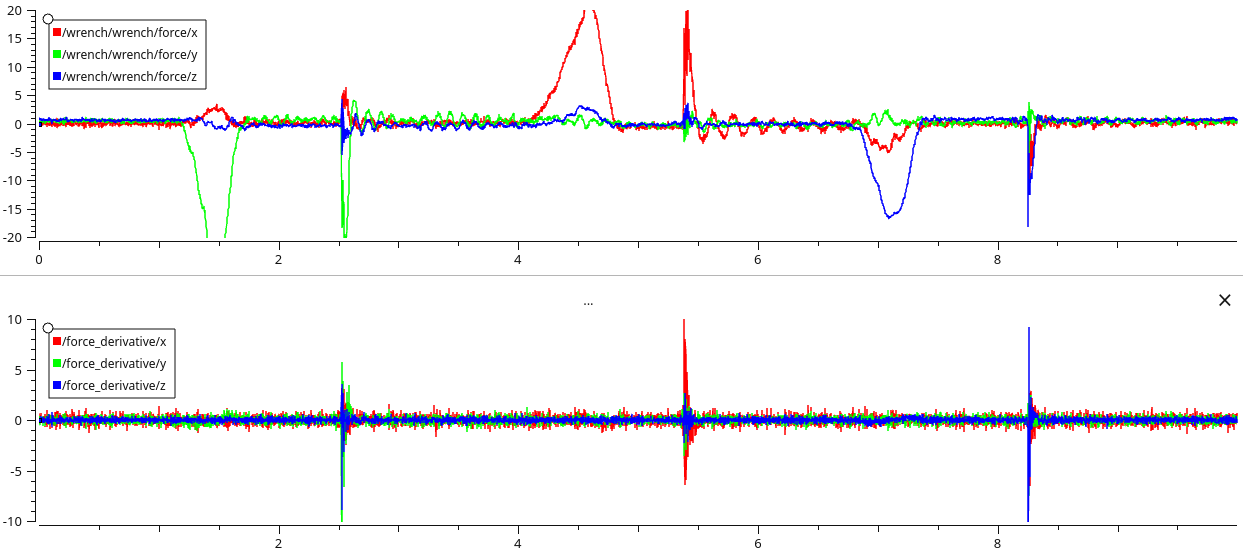
\includegraphics[width=0.9\linewidth]{figs/chp5/taps.png}
    \caption{Result of the compensation architecture applied in a real time test}
    \label{fig:taps}
\end{figure}

\par In the top graph, where raw \ac{ft} values are plotted, a push and a tap are performed in each axis. A push is an amount of force applied slowly, and a tap is the same amount of force, but applied rapidly, like a knock on a door. By looking at the derivative graph on the bottom, it is evident that a tap can be detected just by evaluating the derivative value. 


\subsection{Visual Feedback}

\par Another means of communication with the system is through the 

\begin{figure}[h]
    \centering
    \begin{subfigure}{.2\linewidth}
      \centering
      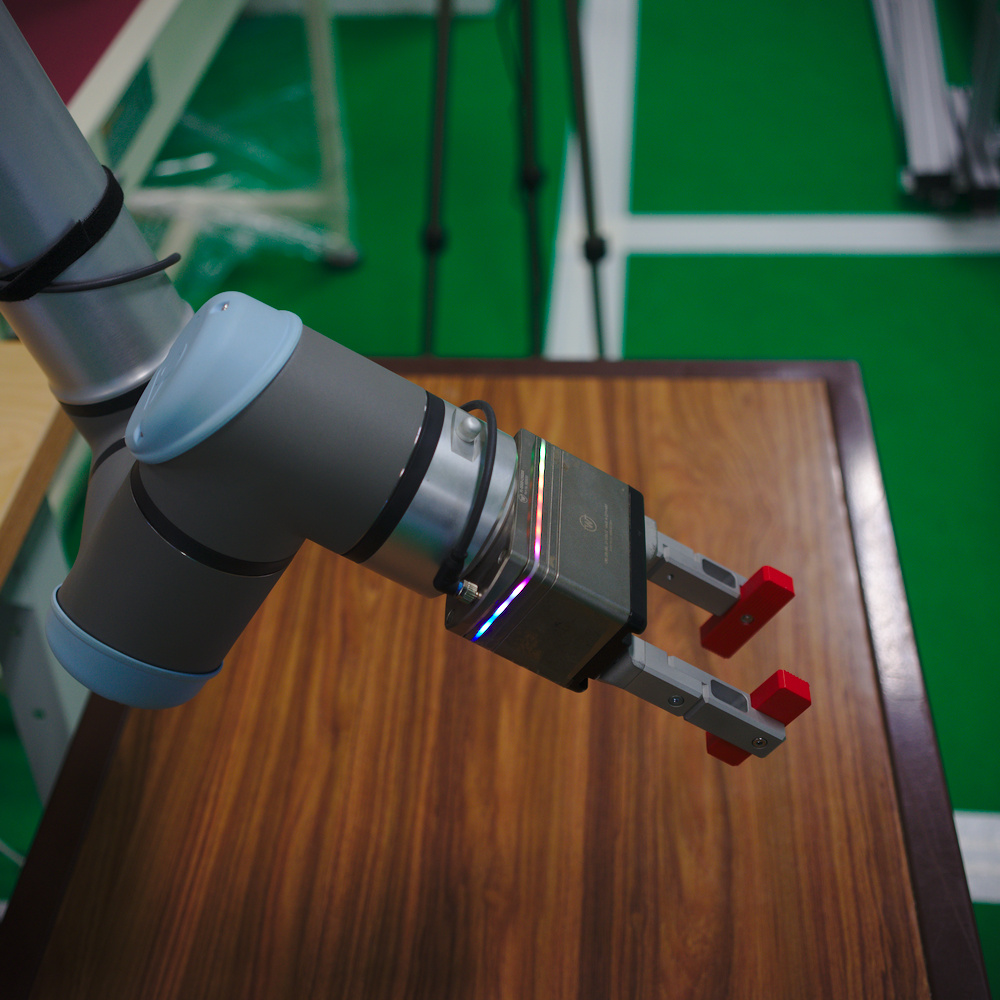
\includegraphics[width=.95\linewidth]{figs/chp5/grip_rgb.jpg}
    \end{subfigure}%
    \begin{subfigure}{.2\linewidth}
      \centering
      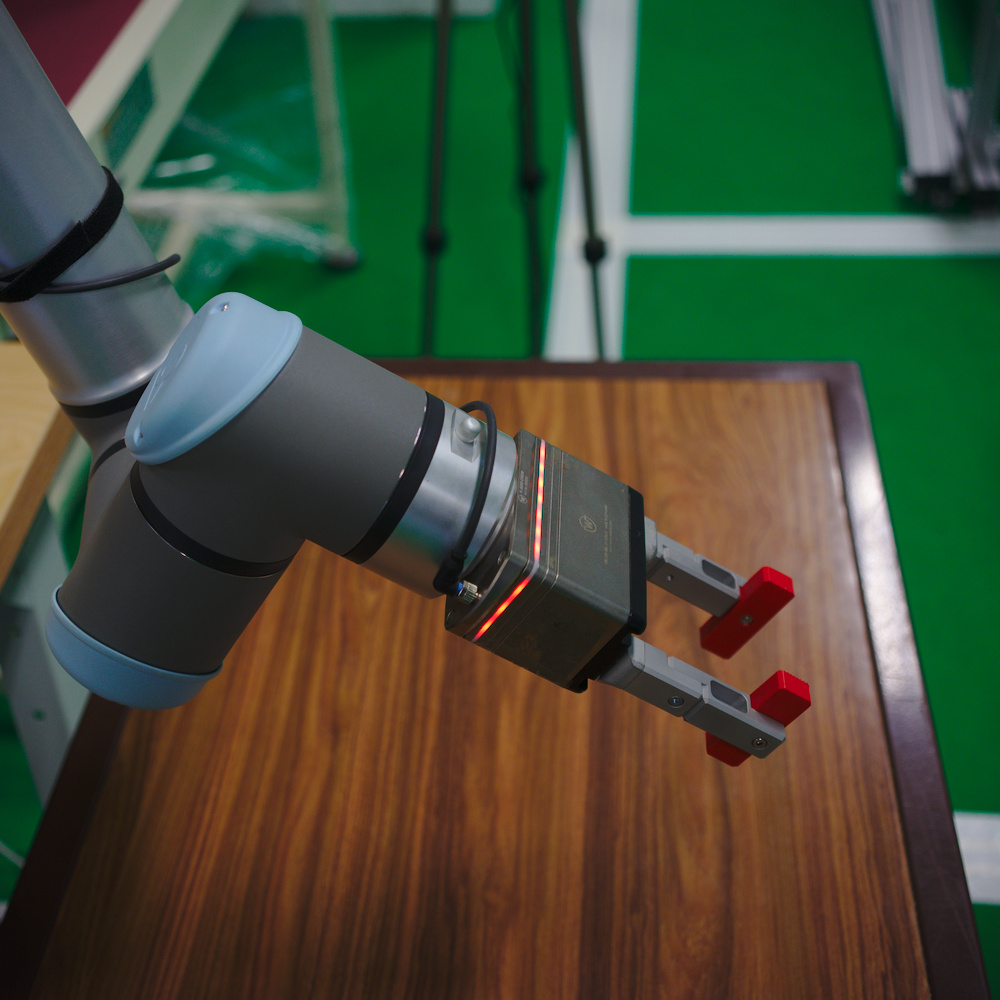
\includegraphics[width=.95\linewidth]{figs/chp5/grip_red.jpg}
    \end{subfigure}%
    \begin{subfigure}{.2\linewidth}
        \centering
        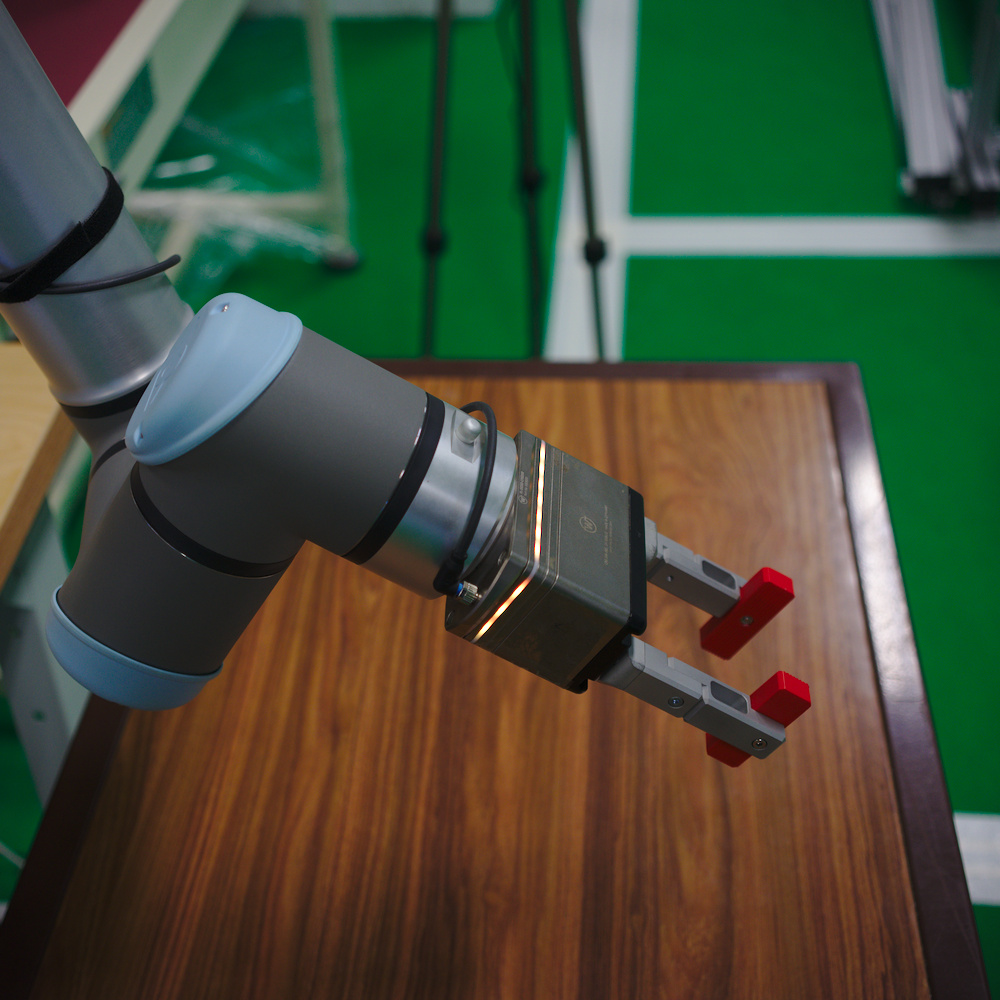
\includegraphics[width=.95\linewidth]{figs/chp5/grip_yellow.jpg}
    \end{subfigure}%
    \begin{subfigure}{.2\linewidth}
        \centering
        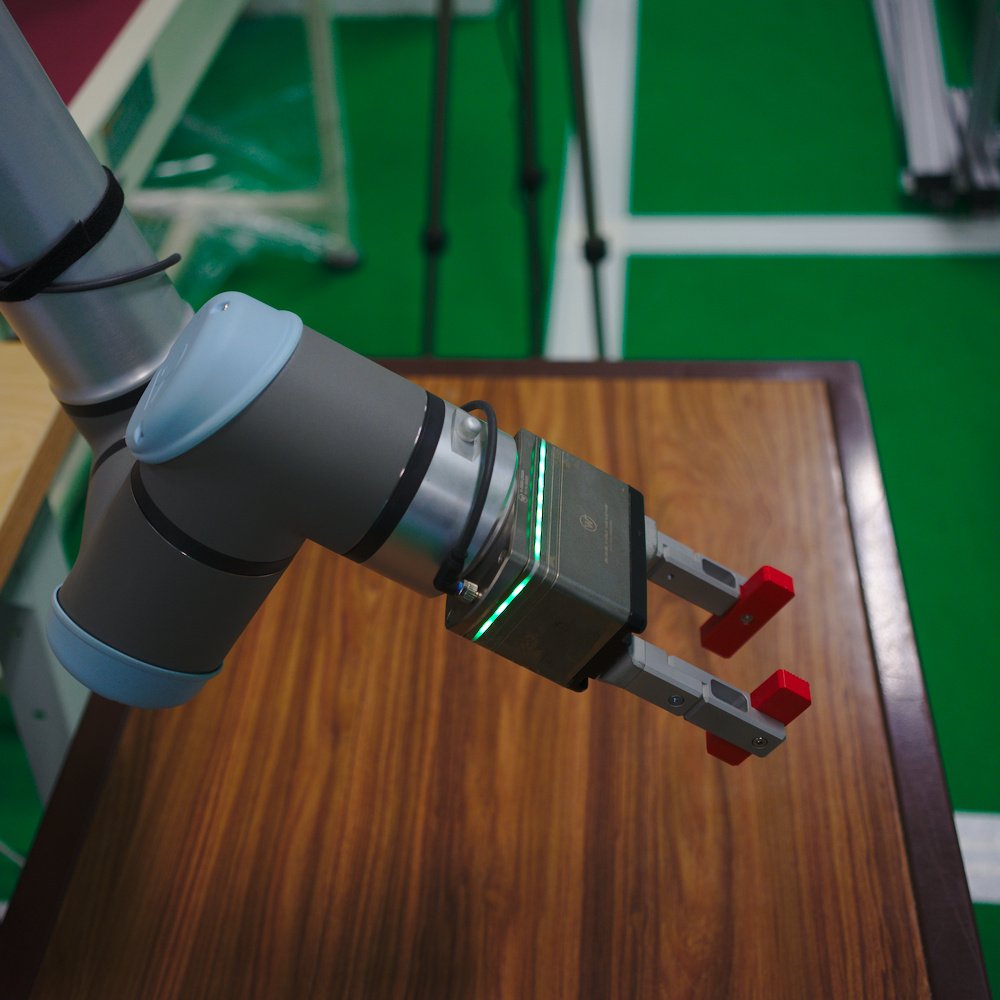
\includegraphics[width=.95\linewidth]{figs/chp5/grip_green.jpg}
    \end{subfigure}%
    \begin{subfigure}{.2\linewidth}
        \centering
        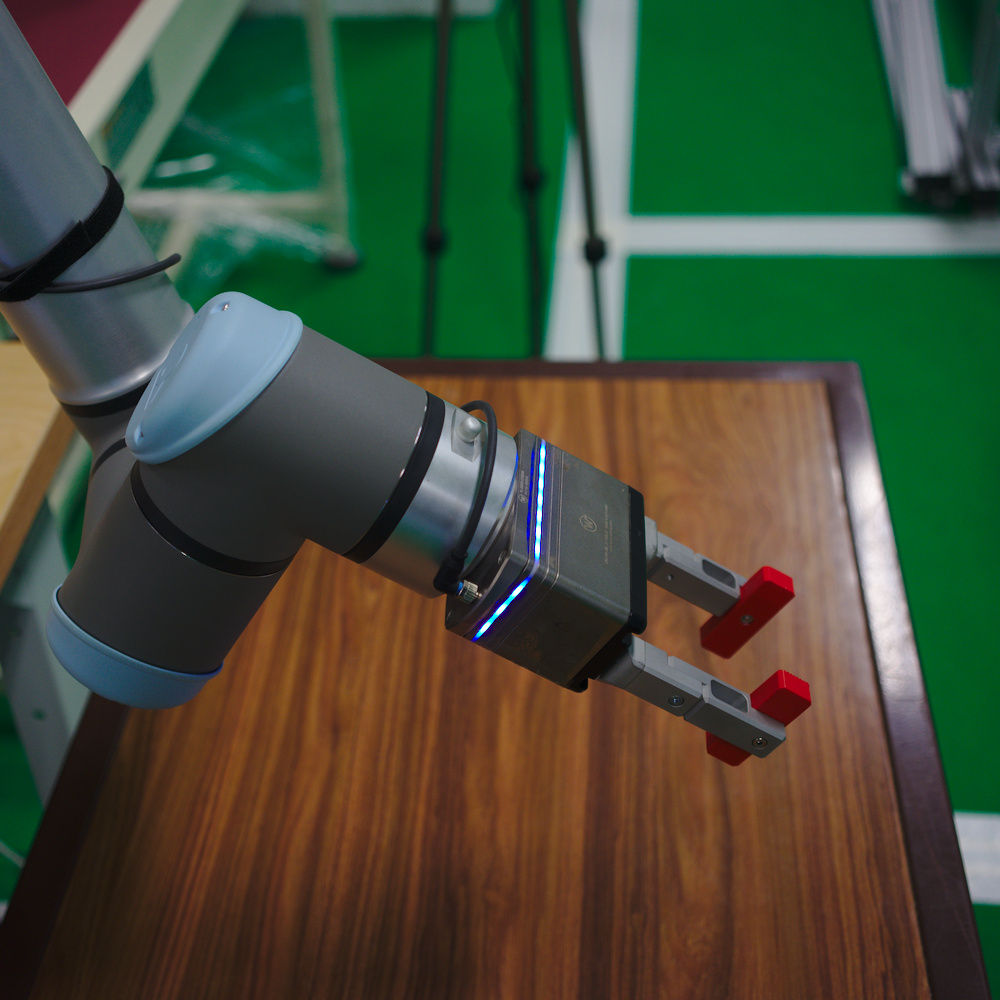
\includegraphics[width=.95\linewidth]{figs/chp5/grip_blue.jpg}
    \end{subfigure}
    \caption{\ac{led} status feedback on the gripper tool}
    \label{fig:gripper_leds}
\end{figure}


\section{Software Tools for \ac{hrc}}
\label{sec:tools-hrc}

\par iris\_sami
\par iris\_cobot
\par other viewers and tools such as plotjuggler integration and smach\_viewer
